\section{Real orders, the finite signed-measure threshold and its atoms}
\label{subunit:sec:main}
\newcommand{\realcut}{\C\setminus[1,\infty)}

The recursive integer-order density is part of a continuous family.
Regularized Hurwitz kernels give the exact finite signed-measure domain,
including its two atomic edges. The construction below supplies the
supercritical part of the later all-positive-order zero theorem.
Write
\[
 A_n(a,b)=\frac{H_{n-1}^{(b)}}{n^a},\qquad
 F_{a,b}(z)=\sum_{n\geq1}A_n(a,b)z^n\quad(|z|<1).
\]
We permit $a=0$ to state the sharp endpoint. Throughout $b>0$;
write $w=a+b$ and $c_n=A_n(a,b)$ in these real-order extensions.

\begin{theorem}[Exact finite-measure domain]
\label{subunit:thm:domain}
For $a\geq0$ and $b>0$, a finite real signed measure $\nu_{a,b}$ on
$[0,1]$ satisfying
\begin{equation}\label{subunit:eq:moments}
 \int_{[0,1]}u^{n-1}\,d\nu_{a,b}(u)=A_n(a,b)
 \qquad(n\geq1)
\end{equation}
exists if and only if
\begin{equation}\label{subunit:eq:domain}
 (a>0\ \hbox{and}\ a+b\geq1)
 \quad\hbox{or}\quad(a=0\ \hbox{and}\ b>1).
\end{equation}
It is unique and has total mass zero. More precisely:
\begin{enumerate}
\item If $a>0$ and $a+b>1$, it has an integrable density
      $\kappa_{a,b}(u)$ with exactly one strict sign change, from
      negative to positive as $u$ increases, at a point $r_{a,b}\in(0,1)$.
\item If $0<b<1$ and $a=1-b$, then
      $\nu_{a,b}=(1-b)^{-1}\delta_1+\kappa_{a,b}(u)\,du$,
      where $\kappa_{a,b}(u)<0$ throughout $(0,1)$.
\item If $a=0$ and $b>1$, then
      $\nu_{0,b}=\zeta(b)\delta_1+\kappa_{0,b}(u)\,du$,
      where $\kappa_{0,b}(u)<0$ throughout $(0,1)$.
\end{enumerate}
In the two atomic cases all positive mass is at one and all negative
mass is in $(0,1)$. Outside \eqref{subunit:eq:domain}, not even a
finite signed measure with arbitrarily many sign changes can satisfy
\eqref{subunit:eq:moments}.
\end{theorem}

\begin{figure}[tbp]
\centering
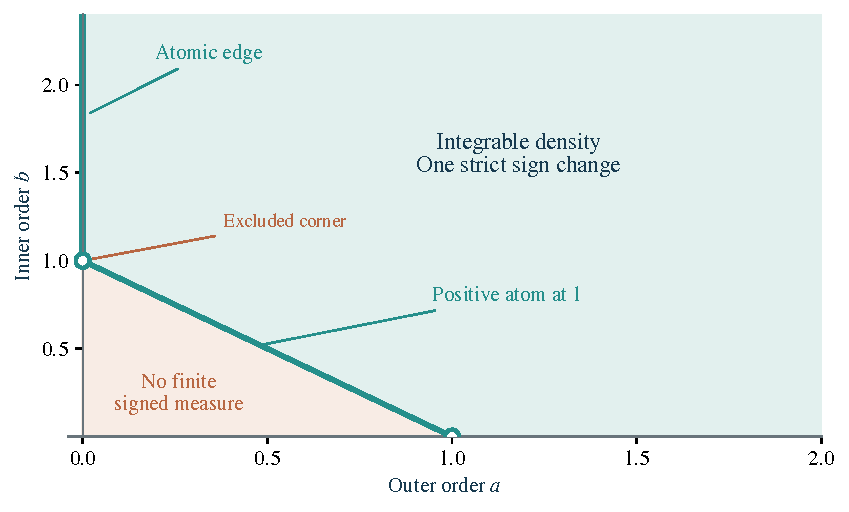
\includegraphics[width=0.8\linewidth]{figures/real_measure_domain.pdf}
\caption{The exact finite signed-measure domain for $a\ge0,b>0$.
The teal edges carry a positive atom at one. The point $(0,1)$ is
excluded, and the horizontal axis $b=0$ is outside the stated domain.
The entire positive quadrant has zero-free principal continuation by
Theorem~\ref{subpick:thm:global}; finite signed-moment existence has the
smaller domain shown here.}
\label{fig:measure-domain}
\end{figure}

\subsection{A regularized positive kernel}

Set
\begin{equation}\label{subunit:eq:q}
 q(t)=\frac1{1-e^{-t}}-\frac1t,\qquad t>0.
\end{equation}
The elementary identities
\[
 q(t)=\frac12+\frac12\coth(t/2)-\frac1t,
 \qquad
 q'(t)=\frac1{t^2}-\frac1{4\sinh^2(t/2)}>0
\]
give $1/2<q(t)<1$, because $\sinh(t/2)>t/2$ and the endpoint
limits are $1/2$ and $1$. In particular $q$ is positive, bounded and
strictly increasing. Also $q(t)=1/2+O(t)$ as $t\downarrow0$.

For later use put $k_v(T)=T^{v-1}/\Gamma(v)$ for $v>0$. The positive convolution satisfies
\begin{align}
 C_{a,b}(T)&=\frac1{\Gamma(a)\Gamma(b)}
 \int_0^T(T-t)^{a-1}t^{b-1}q(t)\,dt
 =k_{a+b}(T)\mathbb E[q(TV)],\quad V\sim\mathrm{Beta}(b,a),
 \label{rw:aux:Cbeta}\\
 \tfrac12 k_{a+b}(T)&<C_{a,b}(T)<k_{a+b}(T),
 \label{rw:aux:Cbounds}\\
 \int_0^\infty e^{-nT}C_{a,b}(T)\,dT
 &=n^{-a}\left(\zeta(b,n)-\frac{n^{1-b}}{b-1}\right)
       \quad(b\ne1).\label{rw:aux:CLaplace}
\end{align}
At $b=1$ the last expression is $n^{-a}(\log n-\psi(n))$.
These identities follow by absolutely convergent convolution integrals.

The classical Hurwitz integral and one elementary subtraction give
\begin{equation}\label{subunit:eq:hurwitz}
 \zeta(b,x)=\frac{x^{1-b}}{b-1}
 +\frac1{\Gamma(b)}\int_0^\infty
              e^{-xt}t^{b-1}q(t)\,dt,
 \qquad x>0,\ b>0,\ b\ne1.
\end{equation}
For $b>1$ this is obtained by splitting $1/(1-e^{-t})=1/t+q(t)$
in the usual Gamma integral. The integral involving $q$ is holomorphic
for $\Re b>0$, so the identity theorem extends the same formula to
$0<b<1$. This is analytic continuation of an absolutely convergent
regularized integral, not subtraction of two divergent real integrals.
The standard starting integral and recurrence are DLMF
25.11.25 and 25.11.4 \cite{intdist:DLMFHurwitz}. For $b=1$ the corresponding formula is
\begin{equation}\label{subunit:eq:digamma}
 \psi(x)=\log x-\int_0^\infty e^{-xt}q(t)\,dt,
\end{equation}
which is DLMF 5.9.13 \cite{rw:DLMFDigamma} and also follows by taking the finite part of
\eqref{subunit:eq:hurwitz} at $b=1$.

For $0<b<1$, we shall use $\zeta(b)<0$. Indeed the alternating
Dirichlet series $\eta(b)$ is positive, while
$\eta(b)=(1-2^{1-b})\zeta(b)$ and $1-2^{1-b}<0$.

\subsection{Explicit densities and their Laplace transforms}

Put $T=-\log u$ and $K_{a,b}(T)=\kappa_{a,b}(e^{-T})$. For
$a>0$, $a+b>1$ and $b\ne1$, define
\begin{align}\label{subunit:eq:generalK}
 K_{a,b}(T)={}&\frac{\zeta(b)T^{a-1}}{\Gamma(a)}
 -\frac{T^{a+b-2}}{(b-1)\Gamma(a+b-1)}\notag\\
 &-\frac1{\Gamma(a)\Gamma(b)}
    \int_0^T(T-t)^{a-1}t^{b-1}q(t)\,dt.
\end{align}
When $b>1$, an equivalent form is
\begin{equation}\label{subunit:eq:largeB}
 K_{a,b}(T)=\frac{\zeta(b)T^{a-1}}{\Gamma(a)}
 -\frac1{\Gamma(a)\Gamma(b)}
   \int_0^T\frac{(T-t)^{a-1}t^{b-1}}{1-e^{-t}}\,dt.
\end{equation}
At $b=1$, define
\begin{align}\label{subunit:eq:bOne}
 K_{a,1}(T)={}&\frac{T^{a-1}}{\Gamma(a)}
       \bigl(\gamma+\psi(a)-\log T\bigr)\notag\\
 &-\frac1{\Gamma(a)}\int_0^T(T-t)^{a-1}q(t)\,dt.
\end{align}
The Gamma factors and the term $\gamma+\psi(a)$ in this last formula
are essential; in particular it reduces at $a=1$ to
$K_{1,1}(T)=-\log(e^T-1)$, agreeing with the original signed kernel.

These functions are integrable against $e^{-T}\,dT$. At zero,
\eqref{subunit:eq:generalK} has only the integrable powers
$T^{a-1}$, $T^{a+b-2}$ and $O(T^{a+b-1})$; the logarithmic factor
in \eqref{subunit:eq:bOne} is likewise integrable for $a>0$.
At infinity all terms have at most polynomial times logarithmic growth.
For $b>1$, the integrability of the convolution in
\eqref{subunit:eq:largeB} at its lower endpoint uses $b>1$ explicitly.

By the Gamma integral and the convolution rule, the Laplace transform
of \eqref{subunit:eq:generalK} is
\begin{align*}
 \int_0^\infty e^{-nT}K_{a,b}(T)\,dT
  &=n^{-a}\left[\zeta(b)-\frac{n^{1-b}}{b-1}
     -\frac1{\Gamma(b)}\int_0^\infty
                         e^{-nt}t^{b-1}q(t)\,dt\right]\\
  &=n^{-a}\bigl(\zeta(b)-\zeta(b,n)\bigr)
   =\frac{H_{n-1}^{(b)}}{n^a}.
\end{align*}
Each convolution interchange is justified absolutely; $q$ is bounded
and the remaining factors have Gamma integrals. Formula
\eqref{subunit:eq:bOne} has Laplace transform
\[
 n^{-a}\left(\gamma+\log n-\int_0^\infty e^{-nt}q(t)\,dt\right)
 =n^{-a}(\gamma+\psi(n))=\frac{H_{n-1}}{n^a}.
\]
Here the Laplace transform of $T^{a-1}\log T$ is obtained by
differentiating the Gamma integral, justified by absolute integrability.
The substitution $u=e^{-T}$ changes $u^{n-1}\,du$ to
$e^{-nT}\,dT$, proving the desired moment normalization. In particular
$n=1$ gives total mass zero.

\subsection{The one-sign-change proof}

For $b>1$, divide \eqref{subunit:eq:largeB} by $T^{a-1}$ and
rescale $t=Tv$:
\[
 T^{1-a}K_{a,b}(T)=\frac{\zeta(b)}{\Gamma(a)}
 -\frac1{\Gamma(a)\Gamma(b)}
  \int_0^1(1-v)^{a-1}v^{b-1}\frac{T^b}{1-e^{-Tv}}\,dv.
\]
For fixed $v>0$, the logarithmic derivative of
$T^b/(1-e^{-Tv})$ is
\[
 \frac bT-\frac{v}{e^{Tv}-1}>\frac{b-1}{T}>0.
\]
Thus the rescaled density is strictly decreasing. Its limit at zero is
$\zeta(b)/\Gamma(a)>0$, and its limit at infinity is $-\infty$.
This proves one strict positive--negative crossing in the $T$ coordinate.

For $b=1$, the rescaled expression is
\[
 \Gamma(a)T^{1-a}K_{a,1}(T)
 =\gamma+\psi(a)-\log T
  -T\int_0^1(1-v)^{a-1}q(Tv)\,dv.
\]
It is strictly decreasing from $+\infty$ to $-\infty$, since $q$ is
positive and increasing. For $0<b<1$, instead divide by
$T^{a+b-2}$ to obtain
\begin{align}\label{subunit:eq:rescaledLowB}
 T^{2-a-b}K_{a,b}(T)={}&
 \frac1{(1-b)\Gamma(a+b-1)}
 +\frac{\zeta(b)}{\Gamma(a)}T^{1-b}\notag\\
 &-\frac{T}{\Gamma(a)\Gamma(b)}
   \int_0^1(1-v)^{a-1}v^{b-1}q(Tv)\,dv.
\end{align}
Now the first term is positive, the second is strictly decreasing
because $\zeta(b)<0$, and the final term is strictly decreasing because
$q$ is positive and increasing. The endpoint limits are a positive
constant and $-\infty$. Thus there is again exactly one strict crossing.
The derivatives of these rescaled expressions are strictly negative;
differentiation is dominated by the same integrable beta weights.
At a zero of $K$, multiplication by the positive rescaling factor does
not affect the sign of its derivative. Reversing $T=-\log u$ gives
the asserted negative--positive sign change and a strictly positive
$u$ derivative at its unique crossing.

\subsection{The critical atom and the exact boundary}

Let $0<b<1$ and $a=1-b$. Replace the middle term of
\eqref{subunit:eq:generalK} by an atom of mass $(1-b)^{-1}$ at $u=1$,
and retain the density
\begin{equation}\label{subunit:eq:criticaldensity}
 K_{1-b,b}(T)=\frac{\zeta(b)T^{-b}}{\Gamma(1-b)}
 -\frac1{\Gamma(1-b)\Gamma(b)}
   \int_0^T(T-t)^{-b}t^{b-1}q(t)\,dt.
\end{equation}
Both terms are strictly negative and integrable against $e^{-T}\,dT$.
Its moments plus the atom are
\[
 \frac1{1-b}+n^{b-1}\left[\zeta(b)
   -\frac1{\Gamma(b)}\int_0^\infty e^{-nt}t^{b-1}q(t)\,dt\right]
 =\frac{H_{n-1}^{(b)}}{n^{1-b}},
\]
by \eqref{subunit:eq:hurwitz}. Thus the measure has total mass zero,
and its negative mass is exactly $(1-b)^{-1}$.

For $a=0$, $b>1$, the formula is especially simple:
\begin{equation}\label{subunit:eq:aZero}
 \nu_{0,b}=\zeta(b)\delta_1+K_{0,b}(-\log u)\,du,
 \qquad K_{0,b}(T)=-\frac{T^{b-1}}{\Gamma(b)(1-e^{-T})}.
\end{equation}
The ordinary Hurwitz integral gives its moments immediately. Its
negative mass is exactly $\zeta(b)$.

Every finite signed measure has bounded moments, since
$|\int u^{n-1}\,d\nu|\leq\|\nu\|_{\mathrm{TV}}$.
If $0<b<1$, elementary integral comparison gives
$H_{n-1}^{(b)}\sim n^{1-b}/(1-b)$, so the moments diverge to
infinity when $a+b<1$. If $a=0,b=1$, they diverge logarithmically.
These are exactly the excluded cases for $a\geq0,b>0$.
Finally, two finite signed measures with the same moments integrate
every polynomial equally; polynomial density in $C([0,1])$ makes the
measures identical. This proves Theorem~\ref{subunit:thm:domain}.

\section{Consequences for complex zeros and angular zeros}

\begin{theorem}[Nonvanishing throughout the finite-measure domain]
\label{subunit:thm:zerofree}
For all parameters in \eqref{subunit:eq:domain}, $F_{a,b}$ has an
analytic continuation to $\mathbb C\setminus[1,\infty)$ and has no
zero there except for its double zero at the origin. Every upper
open semicircle $z=\rho e^{i\theta}$, $0<\rho\leq1$, $0<\theta<\pi$,
has exactly one
simple zero of $\operatorname{Im}F_{a,b}(z)$, and it satisfies
\[
 \arccos\rho<\theta_{a,b}(\rho)<\frac\pi2.
\]
The imaginary part is positive below this angle and negative above
it; its angular derivative at the zero is strictly negative.
In the atomic cases, unit-circle values mean analytic continuation
or Abel boundary values: the original Fourier summands do not tend
to zero, so ordinary Fourier convergence is not asserted.
\end{theorem}

\begin{proof}
The signed transform
\[
 F_{a,b}(z)=z\int_{[0,1]}\frac{d\nu_{a,b}(u)}{1-zu}
\]
follows by geometric expansion in the disk and extends analytically
to the slit plane by uniform domination on compact sets. Let $r$ be
the crossing from Theorem~\ref{subunit:thm:domain}, or let $r=1$ in
the atomic cases. Zero mass gives
\begin{equation}\label{subunit:eq:factor}
 F_{a,b}(z)=\frac{z^2}{1-rz}P_{a,b}(z),\qquad
 P_{a,b}(z)=\int_{[0,1]}\frac{u-r}{1-zu}\,d\nu_{a,b}(u).
\end{equation}
The measure $(u-r)\,d\nu_{a,b}(u)$ is positive and nonzero, including
when $r=1$: its atom disappears but its density is strictly positive
on $(0,1)$. Consequently $\operatorname{Im}P_{a,b}(z)$ has the
strict sign of $\operatorname{Im}z$, while $P_{a,b}(x)>0$ for
$x<1$. Apart from the explicit $z^2$, the factor $(1-rz)^{-1}$ in
\eqref{subunit:eq:factor} is analytic and nonzero on the slit plane. Since $P_{a,b}(0)=A_2=2^{-a}$,
the zero at zero has multiplicity exactly two.

For angular zeros put
\[
 J_\rho(c)=\int_{[0,1]}\frac{d\nu(u)}{1-2\rho cu+\rho^2u^2},
 \qquad
 \operatorname{Im}F(\rho e^{i\theta})
       =\rho\sin\theta\,J_\rho(\cos\theta).
\]
The zero-mass one-crossing sign test holds for our atomic measures as
well: subtract the value of the test function at $r$, and use the
ordered supports of the two signs. It gives $J_\rho(0)<0$.
When $\rho<1$, the kernel at $c=\rho$ is strictly increasing in $u$,
so $J_\rho(\rho)>0$. When $\rho=1$ and the crossing is interior,
separate the two signs before expanding $(1-u)^{-2}$ to obtain
\[
 \lim_{c\uparrow1}J_1(c)
 =\int_{[0,1]}\frac{d\nu(u)}{(1-u)^2}
 =\sum_{n\geq1}n A_n>0,
\]
allowing $+\infty$. The negative part is supported away from one, so
this is the same justified monotone-limit argument as in the original
signed-kernel theorem. In the atomic cases the limiting signed
integral at $c=1$ need not be defined, and we do not use that display.
Instead the limit is $+\infty$ directly: the atom contributes
$M/[2(1-c)]$, and the negative density contributes
$o((1-c)^{-1})$. For the latter assertion, multiply its integral by
$1-c$ and use dominated convergence: the multiplier
$(1-c)/(1-2cu+u^2)$ is bounded by $1$ for $0\leq c<1$ and tends to zero for
every $u<1$. The negative density is integrable and has no atom at one.

For $c'>c$, the quotient of the two kernels has derivative
\[
 \frac{d}{du}\frac{1-2\rho cu+\rho^2u^2}
                         {1-2\rho c'u+\rho^2u^2}
 =\frac{2\rho(c'-c)(1-\rho^2u^2)}
       {(1-2\rho c'u+\rho^2u^2)^2}>0\quad(0<u<1).
\]
At any zero, apply the sign test to the signed measure obtained by
weighting $\nu$ with the positive kernel. It follows that $J_\rho$
is positive at every larger $c$ and negative at every smaller $c$;
this proves uniqueness and the signs. Finally its derivative at its
zero is positive, because the additional factor
$2\rho u/(1-2\rho cu+\rho^2u^2)$ is strictly increasing in $u$.
The angular derivative is therefore
$-\rho\sin^2\theta\,J_\rho'(\cos\theta)<0$.
\end{proof}

\begin{corollary}[Ordinary and analytic boundary values]\label{rw:cor:boundary}
For $a,b>0$ with $a+b>1$, the defining series converges ordinarily
at every $|z|=1,z\ne1$, and equals its analytic continuation. At
$a+b\le1$, or on the axis $a=0,b>0$, its terms do not tend to zero
at those boundary points. There the stated values are analytic or Abel values.
\end{corollary}
\begin{proof}
In the absolutely continuous finite-measure case, expand the finite geometric
sum and use domination of $z(1-(zu)^N)/(1-zu)$ against the total variation;
there is no atom at one. Harmonic asymptotics give a positive nonzero limit
or unbounded coefficients in the remaining cases, so the term test fails.
The axis formula and the subsequent Stieltjes factorization still give
well-defined continuation and radial Abel limits away from the cut.
\end{proof}
